\documentclass{beamer}
\mode<presentation> {
	\usetheme{Hannover}
}
\usecolortheme{default}

\usepackage{amsmath,amssymb}
\usepackage[utf8]{inputenc}
\usepackage[ngerman]{babel}
\usepackage[T1]{fontenc}
\usepackage{siunitx}
\usepackage{lmodern}
\usepackage{graphicx}
\usepackage{subfigure}

\beamertemplatenavigationsymbolsempty

\author{Stefan Kull, Roy Seitz}
\title{Besselfunktion - Wo ist die zweite Lösung?}

\newenvironment{slide}
{\begin{frame}[environment=slide]
	\frametitle{\insertsection}
	\framesubtitle{\insertsubsection}}
{\end{frame}}


\begin{document}
	
	\begin{slide}
		\titlepage
	\end{slide}
	
%	\begin{slide}
%		\tableofcontents
%	\end{slide}
	
\section{Bekannt}	
\subsection{Bessel'sche Differentialgleichung}	
	\begin{slide}
		Lösungen der Differentialgleichung
		$$ z^2w''+zw'+(z^2-\nu^2)w=0 $$
		in folgender Form
		$$
		w(z)=J_\nu(z)=z^\varrho\sum_{k=0}^{\infty}a_kz^k 
		$$ $$
		\varrho=\pm\nu
		$$
	\end{slide}
	
%\subsection{Indexgleichung und $\varrho$}
%	\begin{slide}
%		Indexgleichung
%		$$\varrho(\varrho-1)+p_0\varrho+q_0=0$$
%		Für die Besselgleichung:
%		$$p_0=1, q_0=-\nu^2$$
%		$$\varrho=\pm\nu $$
%	\end{slide}

\subsection{Besselfunktion 1. Art}
	\begin{slide}
		\centering
		$$J_\nu(z)=z^\varrho\sum_{k=0}^{\infty}a_kz^k$$
		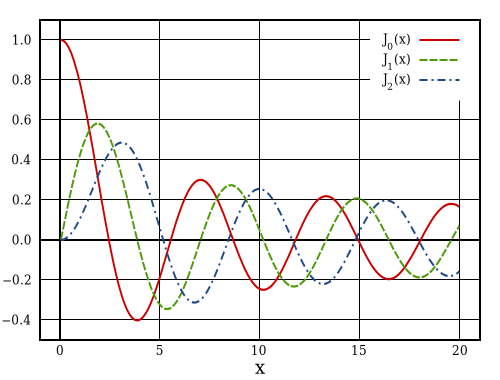
\includegraphics[scale=0.5]{Bilder/Bessel_Functions_1st_Kind.pdf}
	\end{slide}

\section{Problem}
\subsection{Lineare Abhängigkeit und doppelte $\varrho$}
	\begin{slide}
		Lineare Abhängigkeit bei ganzzahligen $\nu\in\mathbb{Z}\setminus\{0\}$:
		$$J_\nu(z) = J_{-\nu}(-z)$$
		Bei $\nu=0$ nur eine Lösung
		$$\varrho=\pm 0\Rightarrow J_0(z)$$
	\end{slide}
	
\subsection{Wo ist die 2. Lösung?}
	\begin{slide}		
		DGL 2. Ordnung $\Rightarrow$ 2 Lösungen.
		
		Wie findet man die zweite Lösung?
		
	\end{slide}

\section{Ziel}

\subsection{Besselfunktion 2. Art}
\begin{slide}
	\centering
	$$Y_\nu(x)=x^\varrho\sum_{k=-\infty}^{\infty}a_kx^k+aJ_\nu(x)\log(x)$$
	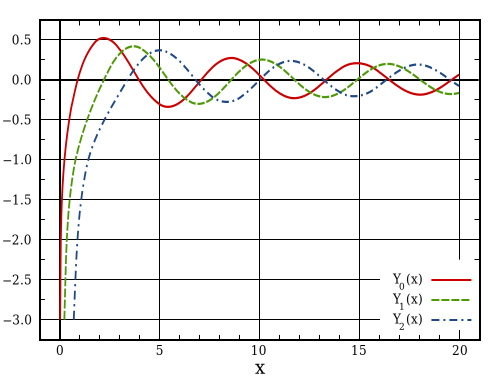
\includegraphics[scale=0.5]{Bilder/Bessel_Functions_2nd_Kind.pdf}
\end{slide}

\begin{slide}
	$$J_\nu(x)=x^\varrho\sum_{k=0}^{\infty}a_kx^k$$
	$$Y_\nu(x)=x^\varrho\sum_{k=-\infty}^{\infty}a_kx^k+aJ_\nu(x)\log(x) $$
	\begin{figure}
		\subfigure{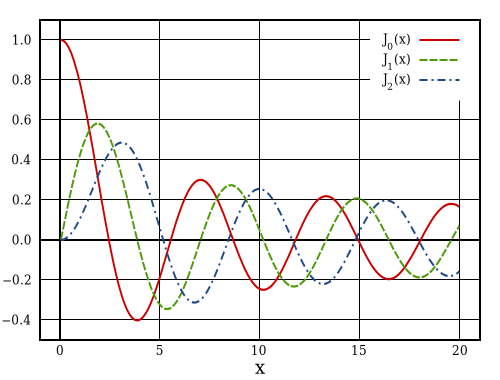
\includegraphics[width=0.49\textwidth]{Bilder/Bessel_Functions_1st_Kind.pdf}}
		\subfigure{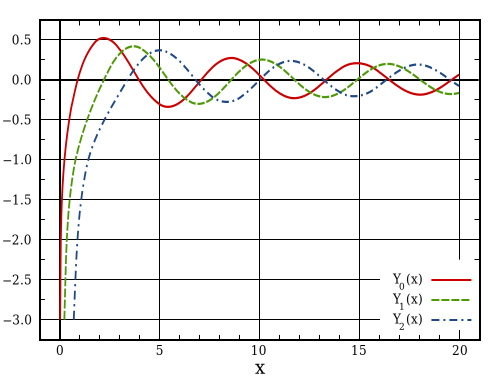
\includegraphics[width=0.49\textwidth]{Bilder/Bessel_Functions_2nd_Kind.pdf}}			
	\end{figure}
\end{slide}

\section{Benötigte Werkzeuge}
	\begin{slide}
		\begin{itemize}
			\item Laurent-Reihe
			$$\mathcal{L}(z)=\sum_{k=-\infty}^{\infty}a_kz^k $$
			\item Analytische Fortsetzung
			\item Etwas (lineare) Algebra\ldots
		\end{itemize}
	\end{slide}
	
\end{document}
